\documentclass[11pt, oneside]{article} 
\usepackage{geometry}
\geometry{letterpaper} 
\usepackage{graphicx}
	
\usepackage{amssymb}
\usepackage{amsmath}
\usepackage{parskip}
\usepackage{color}
\usepackage{hyperref}

\graphicspath{{/Users/telliott/Github/precalculus/fig/}}
% \begin{center} \includegraphics [scale=0.4] {gauss3.png} \end{center}

\title{Arcs of a circle}
\date{}

\begin{document}
\maketitle
\Large
\label{sec:generalized_arc}

We have previously established some central facts about circles including Thales' theorem about the angle intercepting a half-arc of the circle being a right angle.  We will need some of these results later.

Now, we do more.  We can generalize the results for all arcs.  

\subsection*{arcs encompassing diameter}

The examples so far directly contain the diameter in some way. 

Consider the arc swept out by the angle $s$ in this figure (left panel).

\begin{center} 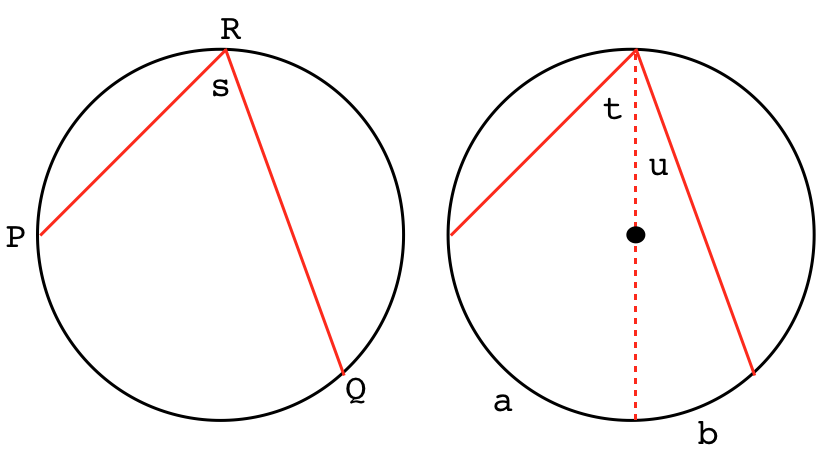
\includegraphics [scale=0.4] {arcs1.png} \end{center}

We can prove that the measure of the angle $s$ is equal to one-half the arc swept out between P and Q.

Draw the diameter (right panel):
By our previous work:

\[ 2t = a, \ \ \ \ \ \ 2u = b \]
and
\[ s = t + u \]
\[ 2s = 2t + 2u = a + b \]
\[ s = \frac{1}{2} \ (a + b) \]

Thus, we have proved the theorem for

$\bullet$ \ the special case where the arc is a diameter of the circle

$\bullet$ \ the general case where the diameter is one chord flanking the arc

$\bullet$ \ another general case where the arc includes the diameter.

\subsection*{arc without diameter}

However, the theorem is true even if the angle does not include the diameter.  We use subtraction.

\begin{center} 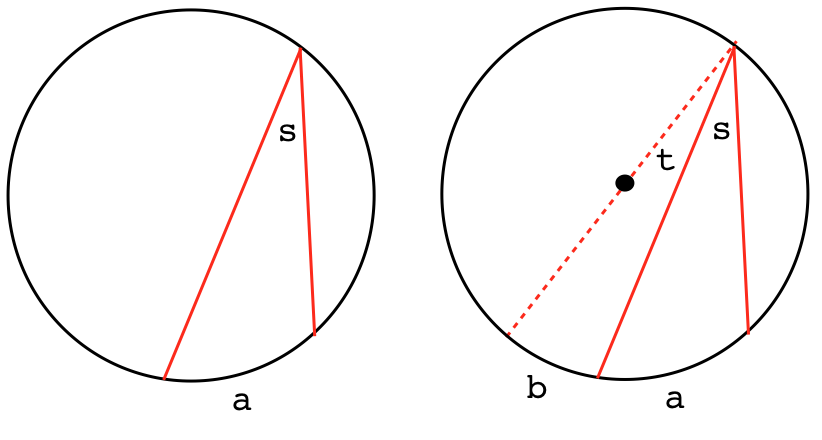
\includegraphics [scale=0.4] {arcs2.png} \end{center}

On the right, draw the diameter.  There are two arcs which include the diameter:  one with angle $t$ and one with angle $s+t$.  We obtain the generalized arc with angle $s$ by subtracting the result for $t$ from that for $s + t$.

\[ 2t = b \]
\[ 2(s+t) = a + b \]
Subtract:
\[ 2s = a \]
\[ s = \frac{1}{2} \ a \]

As a corollary, any two angles with vertexes (vertices) on the circle that cut off the same arc are equal.  In the figure below, $s = s'$ (left panel)
\begin{center} 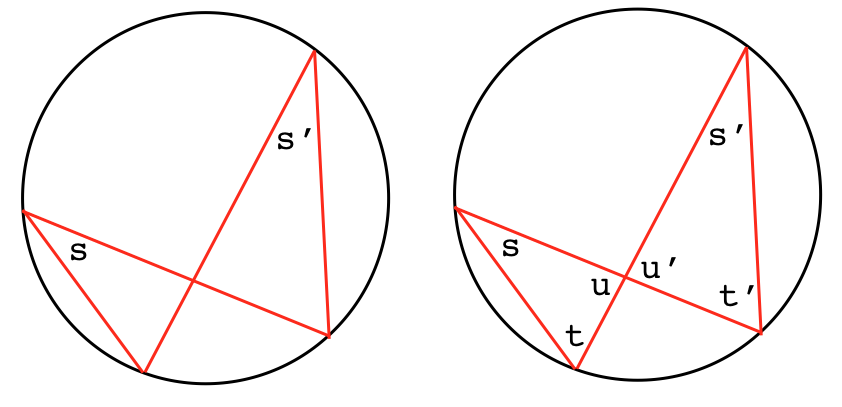
\includegraphics [scale=0.4] {arcs3.png} \end{center}

and $t = t'$ (right panel).  So $u = u'$ by both the vertical angle theorem and by of the triangle sum theorem.  Therefore, the two triangles are similar.  We will come back to this.

\subsection*{Intersecting chords}
Given two chords, to prove:

\[ s = \frac{1}{2} (a + b) \]
$s$ is the average of the two arc lengths.

\begin{center} 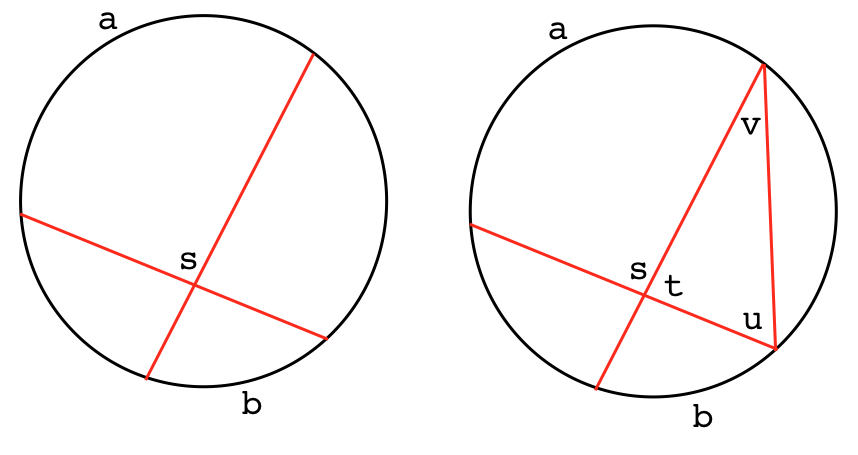
\includegraphics [scale=0.4] {arcs4.png} \end{center}

Solution:  Draw a triangle (right panel, above).
\[ 2v = b \]
\[ 2u = a \]
The external angle is the sum of the two opposing interior angles.
\[ s = u + v = \frac{1}{2} \ (a + b) \]

\subsection*{Tangent and secant}

Rather than having all three points on the circle, one point is now outside. We have the same arc swept out by the endpoints ($a$), but the included angle is smaller, and there is a new small piece of arc length $b$.

\begin{center} 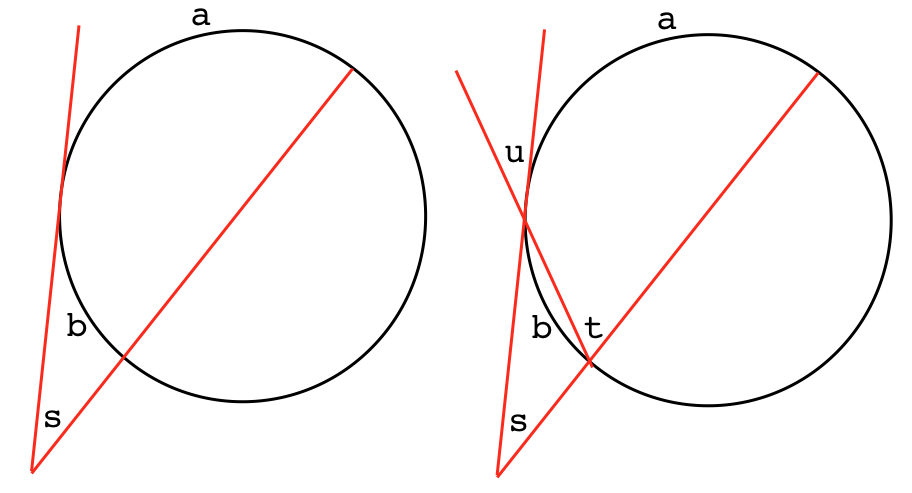
\includegraphics [scale=0.4] {arcs5.png} \end{center}

To prove:
\[ s = \frac{1}{2} (a - b) \]

Solution:
Draw the triangle.  By our previous work:
\[ 2t = a \]
By the vertical angle theorem the unlabeled angle inside the triangle is equal to $u$ and it subtends arc $b$ so
\[ 2u = b \]
By the exterior angle theorem
\[ t = s + u \]
\[ s = t - u = \frac{1}{2} \ (a - b) \]

\subsection*{Chord segments}

Finally, there is a simple algebraic relationship between chord segments. Draw two chords of the circle.

\begin{center} 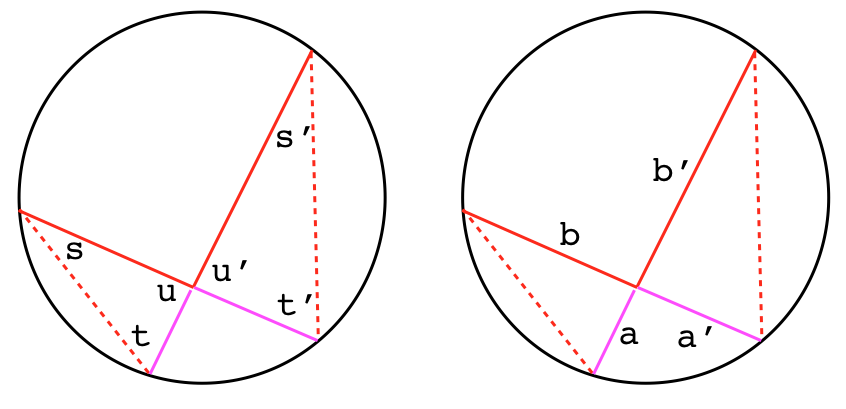
\includegraphics [scale=0.4] {arcs6.png} \end{center}

Draw the two triangles.  The angles are equal to their primed counterparts ($s = s'$ and $t = t'$ because they subtend equal arcs, while $u = u'$ by the vertical angle theorem).  

Therefore, the triangles are similar.  Similar sides are indicated by color or style, and labeled with primes in the right panel, where the letters refer to the sides.

\[ a/b = a'/b' \]
\[ ab' = a'b  \]

For any two chords that cross in a circle, the products of the chord segments are equal.  We use this later in looking at the spherical cap.

We can prove a similar theorem about chords extended from a circle.

\begin{center} 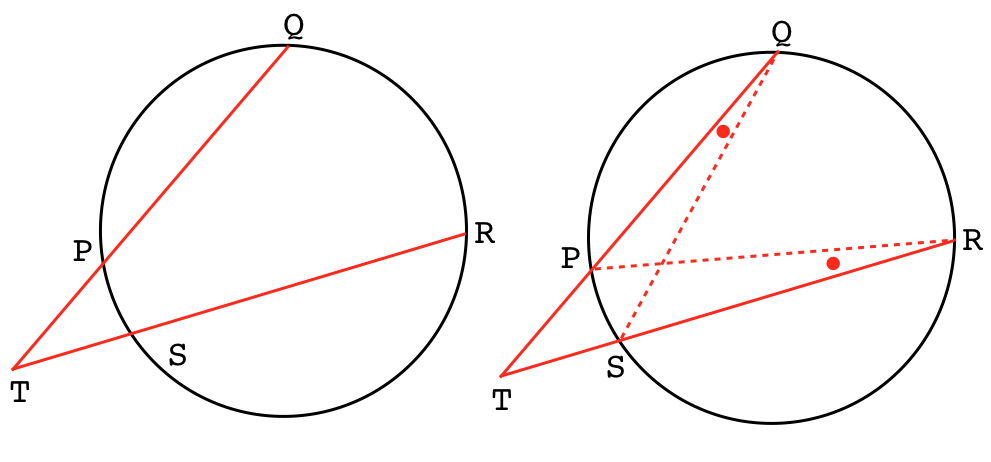
\includegraphics [scale=0.4] {arcs7.png} \end{center}

The two angles marked with red dots subtend the same arc, so they are equal.  The angle at vertex $T$ is shared, therefore $\triangle QST \cong \triangle PRT$.

By similar triangles we have that
\[ \frac{TP}{TS} = \frac{TQ}{TR} \]
\[ TP \cdot TR = TS \cdot TQ \]

\subsection*{cyclic quadrilateral}

\begin{center} 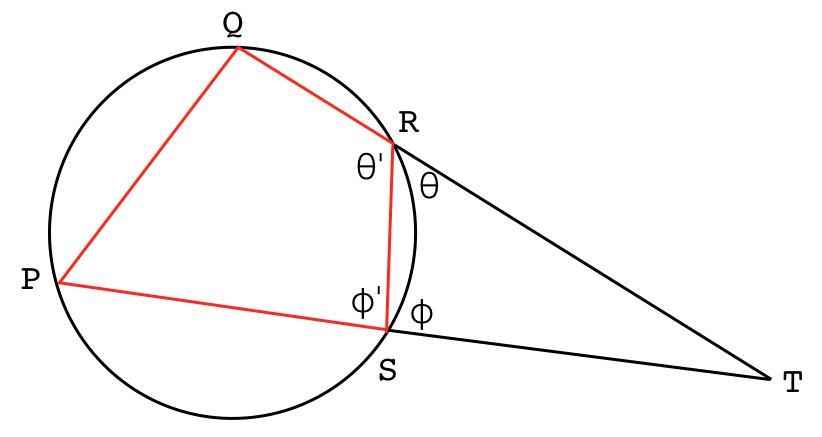
\includegraphics [scale=0.4] {cyclic_quad.png} \end{center}

A cyclic quadrilateral is a four-sided figure where all four vertices lie in a circle.  Surprisingly, the two triangles in the figure are similar.

To prove:  $\triangle PQT \sim \triangle RST$.

The supplementary angle $\phi'$ subtends arc $PQR$, therefore $\phi$ is equal to the angle at vertex $Q$, which subtends arc $PSR$.  

Similarly, $\theta'$ subtends arc $QPS$, therefore $\theta$ is equal to the angle at vertex $P$.

$\square$






\end{document}